%\documentclass[showpacs,preprintnumbers,amsmath,amssymb,superscriptaddress,aip]{revtex4-1}
\documentclass[letter,scriptaddress,twocolumn, prl,showkeys]{revtex4}
\usepackage{graphicx}
%\usepackage{amssymb}
%\setlength{\parindent}{0in}

% General Latex  --------------------------------------------------
\def\beq{\begin{equation}}
\def\eeq{\end{equation}}
\def\beqar{\begin{eqnarray}}
\def\eeqar{\end{eqnarray}}
\def\nn{\nonumber}
\def\ol{\overline}
\def\para{\parallel}

% Operators  ------------------------------------------------------
\newcommand{\diff}[2]{\frac{d#1}{d#2}}
\newcommand{\diffs}[2]{\frac{d^2#1}{d#2^2}}
\newcommand{\pdiff}[2]{\frac{\partial#1}{\partial#2}}
\newcommand{\pdiffs}[2]{\frac{\partial^2#1}{\partial#2^2}}
\newcommand{\pdiffxy}[3]{\frac{\partial^2#1}{\partial#2 \partial#3}}
\newcommand{\pdt}{\partial_t}
\newcommand{\pdr}{\partial_r}
\newcommand{\pdth}{\partial_\theta}
\newcommand{\pdrr}{\partial^2_r}

\newcommand{\enum}[2]{{#1}\times10^{#2}} % 4.2x10^{3} = \enum{4.2}{3}

\newcommand{\vect}[1]{{\bf #1}}
%\newcommand{\vect}{\overrightarrow}
%\newcommand{\vect}{\vec}
\def\div{\nabla\cdot}
\def\grad{\nabla}
\def\curl{\nabla\times}
\newcommand{\gradpar}{\grad_\parallel}
\newcommand{\gradperp}{\grad_\perp}
\newcommand{\gradr}{\grad_r}
\newcommand{\defeq}{\ensuremath{\stackrel{\text{\tiny def}}{=}}}

\newcommand{\savg}[1]{\left<{#1}\right>}
\newcommand{\vavg}[1]{\left<{#1}\right>_V}
\newcommand{\thavg}[1]{\left<{#1}\right>_\theta}

% Variable names  -------------------------------------------------
\newcommand{\vpar} {v_\parallel}
\newcommand{\Apar} {A_\parallel}
\newcommand{\jpar} {j_\parallel}
\newcommand{\kpar} {k_\parallel}
\newcommand{\kperp} {k_\perp }
\newcommand{\vperp} {v_\perp }
\newcommand{\kthe}{k_\theta}

\newcommand{\Evec}{\ensuremath{\boldsymbol{{\rm E}}}}
\newcommand{\Bvec}{\ensuremath{\boldsymbol{{\rm B}}}}
\newcommand{\Jvec}{\ensuremath{\boldsymbol{{\rm J}}}}
\newcommand{\Fvec}{\ensuremath{\boldsymbol{{\rm F}}}}
\newcommand{\fvec}{\ensuremath{\boldsymbol{{\rm f}}}}
\newcommand{\vE}{\ensuremath{\boldsymbol{{\rm v}_{E}}}}
\newcommand{\bo}{\ensuremath{\boldsymbol{{\rm b}_0}}}
\newcommand{\bvec}{\ensuremath{\boldsymbol{{\rm b}}}}
\newcommand{\xvec}{\ensuremath{\boldsymbol{{\rm x}}}}
\newcommand{\yvec}{\ensuremath{\boldsymbol{{\rm y}}}}
\newcommand{\zvec}{\ensuremath{\boldsymbol{{\rm z}}}}
\newcommand{\vvec}{\ensuremath{\boldsymbol{{\rm v}}}}
\newcommand{\jvec}{\ensuremath{\boldsymbol{{\rm j}}}}

\newcommand{\bxgp}{\bvec\times\gradperp}

\newcommand{\vve}{\ensuremath{\boldsymbol{{\rm v}}_{e}}}
\newcommand{\vvi}{\ensuremath{\boldsymbol{{\rm v}}_{i}}}
\newcommand{\vpe}{v_{\parallel e}}
\newcommand{\vpi}{v_{\parallel i}}
\newcommand{\vvE}{\ensuremath{\boldsymbol{{\rm v}}_{E}}}
\newcommand{\vvD}{\ensuremath{\boldsymbol{{\rm v}}_{D}}}

\newcommand{\nuei}{\nu_{ei}}
\newcommand{\nuii}{\nu_{ii}}
\newcommand{\nue}{\nu_{e}}
\newcommand{\nuen}{\nu_{en}}
\newcommand{\nuin}{\nu_{in}}
\newcommand{\kpe}{\kappa_{\parallel e}}

\newcommand{\rs}{\rho_{s}}
\newcommand{\ri}{\rho_{i}}
\newcommand{\wci}{\Omega_{i}}
\newcommand{\wcix}{\Omega_{ix}}
\newcommand{\wce}{\Omega_{e}}
\newcommand{\tomega}{\tilde\omega}
\newcommand{\Isat}{I_{\rm sat}}
\newcommand{\fmie}{\frac{m_i}{m_e}}
\newcommand{\fmei}{\frac{m_e}{m_i}}


% Often used dimensions
\newcommand{\cm}{\rm cm}
\newcommand{\mm}{\rm mm}
\newcommand{\cmn}{{\rm cm}^{-3}}
\newcommand{\mn}{{\rm m}^{-3}}
\newcommand{\eV}{\rm eV}
\newcommand{\G}{\rm G}
\newcommand{\T}{\rm T}



\begin{document}

\title{}

\author{B. Friedman}
\email{friedman@physics.ucla.edu}

\author{T.A. Carter}

\affiliation{Department of Physics and Astronomy, University of California, Los Angeles, California 90095-1547, USA}



\begin{abstract}

\end{abstract}

\maketitle

\section{Introduction}

Turbulence in magnetically confined plasmas is almost always attributed to linear instabilities. The calculation of linear instabilities through normal mode analysis
-- the calculation of eigenvalues and eigenvectors of a linearized dynamical system -- has successfully predicted the onset criterion for many MHD and micro-instabilities.
Nevertheless, it is well-known in the hydrodynamics community that normal mode analysis fails at predicting turbulent onset for a large class of experiments that are deemed to have
subcritical turbulence. Subcritical turbulence is certainly possible in plasmas, and several instances have been studied in the 
past~\cite{waltz1985,scott1990,scott1992,nordman1993,biskamp1995,drake1995,camargo1998,krommes1999,scott2002,camporeale2009,camporeale2010,schekochihin2012,highcock2012}. 
For the most part, however, normal mode analysis dominates plasma turbulence prediction despite the fact that it is not useful in all instances.

Since the hydrodynamics community has long studied subcritical turbulence, it has much to offer in terms of understanding the phenomenon. Most significantly,
in the early 1990's, Trefethen and others attributed the failure of normal mode analysis in predicting subcritical turbulent onset to the non-normality of linear operators of
dynamical systems~\cite{trefethen1993,schmid2007}. A non-normal operator has 
eigenvectors that are not orthogonal to one another. One consequence of eigenvector nonorthogonality is that even when all eigenvectors decay exponentially under linear evolution, 
superpositions of eigenvectors can grow, albeit transiently.
In other words, certain fluctuations of the laminar state can access free energy from background gradients even though normal mode fluctuations cannot.
When combined with nonlinear effects, this allows for sustained subcritical turbulence by a bootstrapping process.
Such behavior is obscured by traditional normal mode analysis, which only effectively describes the long time asymptotic behavior of fluctuations under  
action of the linear operator. Transient growth, which can dominate turbulent evolution, can be discovered only through non-modal calculations.

Non-modal analysis generally employs tools such as pseudospectra and maximum possible transient growth curves, which have been used to successfully explain why turbulence is subcritical in various
systems. However, to our knowledge, they have not been used to predict onset criteria in subcritical systems (e.g. the transition Reynold's number in pipe flows), although non-normal
turbulent arguments have been applied in generating amplitude versus Reynold's number scalings for turbulent onset.
This paper takes up the task of developing a new approach to understand turbulent properties using only non-modal linear calculations with the goal of 
ultimately making quantitative predictions.  Our approach is to calculate an average growth rate of turbulent fluctuations due to linear processes, specifically due to transient growth.  We model the
turbulent steady state as a series of processes:  (1) the turbulence starts as a spatially random state, (2) linear transient growth deterministically amplifies the turbulent energy (or
decrease it in wavenumber ranges where linear damping dominates), (3) nonlinear transfer sets in at a specified timescale, terminating the
transient growth process and re-randomizing the turbulent state (at which point the cycle repeats).    Optimally, the timescale for the final step would be the
nonlinear decorrelation time of the turbulent system, but in order to enable predictive capability, we employ critical balance
arguments to use a characteristic \emph{linear} time. The procedure ultimately produces a growth rate that can be used
to predict turbulent properties such as saturation levels and transport rates through mixing length arguments.

\section{Non-Normality of the Hasegawa-Wakatani Model}

Before employing the non-modal technique, we explore the effect of non-normality in the well-known and well-analyzed Hasegawa-Wakatani (HW) model~\cite{hasegawa1983}. 
We consider both the original 2D and the extended 3D~\cite{biskamp1995} versions of the model in a straight, unsheared magnetic field. 
The HW model consists of two equations for the density $n$ and the electrostatic potential $\phi$. The 3D version of the model is

\beqar
\label{n_eq}
\pdiff{n}{t} = - {\mathbf v_E} \cdot \grad n - \kappa \pdiff{\phi}{y} + \xi \gradpar^2 (n - \phi) - D \gradperp^4 n, \\
\label{phi_eq}
\pdiff{\gradperp^2 \phi}{t} = - {\mathbf v_E} \cdot \grad (\gradperp^2 \phi) + \xi \gradpar^2 (n - \phi) - D \gradperp^6 \phi
\eeqar
The normalizations are $\phi \to e \phi/T_e, n \to n/n_0, \grad \to \rho_s \grad , x,y,z \to x,y,z/\rho_s, t \to \omega_{ci} t $. Additionally,
$\mathbf{v_E} = \mathbf{b} \times \grad \phi$, $\xi = 4 \pi \omega_{ce}/\nu_{ei}$, 
and $\kappa = \rho_s/L_n$, where $L_n$ is the density scale length. The terms $D \gradperp^4 n$ and $D \gradperp^6 \phi$ are artificial hyper-diffusion and hyper-viscosity used to dissipate
energy on small scales. We set $D \to 10^{-5}$ except when otherwise indicated.
We associate the direction along $\mathbf{B}$ as the parallel or $z$ direction. The direction perpendicular $\mathbf{B}$ that
points opposite the density gradient is defined as the $x$ direction, and the $y$ direction is taken perpendicular to both of these.

In the analysis and numerical simulations, which we perform with the BOUT++ code~\cite{dudson2009}, we use periodic boundary conditions in
the $y$ and $z$ directions with zero-value boundaries in the $x$ direction. We use a domain size of $64 \rho_s \times 64 rho_s \times 300 \rho_s$.
For the 2D version of the model, we replace $-\xi \gradpar^2$ by $\alpha = k_z^2 \xi = 4 \pi k_z^2 \rho_s^2 \omega_{ce} /\nu_{ei}$, 
which is commonly known as the adiabaticity parameter~\cite{camargo1995,camargo1998}. Additionally we use a domain size of $50 \rho_s \times 50 \rho_s$.
In numerical simulations, the turbulence can laminarize due to the build-up of $k_y=0$ density and potential structures~\cite{biskamp1995}. To prevent this, we subtract out the $k_y=0$
$n$ and $\phi$ components, which is the equivalent of adding source terms to Eqs.~\ref{n_eq} and~\ref{phi_eq}~\cite{friedman2012b}.

The degree of non-normality of the linear operator in the HW model is largely a function of the adiabaticity parameter~\cite{camargo1998}, or in the 3D case, of $\xi \gradpar^2$. 
Note that a matrix is normal if it commutes with its adjoint: $\mathbf{D} \mathbf{D}^\dagger = \mathbf{D}^\dagger \mathbf{D}$ for $\mathbf{D}$ normal. 
The HW model has a normal linear operator in the limit of $\alpha, \xi \gradpar^2 \to \infty$. 
To see this, we first transform the linear operator into a linear matrix by using a Fourier decomposition. Because we use a zero-value boundary condition in the $x$ direction, the
Fourier decomposition takes the form:

\beq
\label{fourier_form}
f_k = \int_0^{L_x,L_y,L_z} f(\mathbf{r}) \ {\rm sin} \left( k_x x \right) e^{i k_y y + i k_z z} d\mathbf{r}
\eeq
where $k_x = \pi l/L_x, k_y = 2 \pi m/L_y, {\rm and } \ k_z = 2 \pi n/L_z$ with $l, m, {\rm and } \ n$ integers.
The result for the 3D model is an equation for each mode $k = (k_x,k_y,k_z)$:

\beqar
\label{fourier_eqn}
\frac{\partial}{\partial t} \left( \begin{array}{cc} n_k \\ \phi_k \end{array} \right) = \mathbf{A}_k \left( \begin{array}{cc} n_k \\ \phi_k \end{array} \right) + \mathbf{N}_k \left( \begin{array}{cc} n_k \\ \phi_k \end{array} \right), \\ \nonumber \\
\label{A_k}
\mathbf{A}_k = \left( \begin{array}{cc} -\xi k_z^2 - D k_\perp^4 & -i \kappa k_y + \xi k_z^2 \\  \xi \frac{k_z^2}{k_\perp^2} & - \xi \frac{k_z^2}{k_\perp^2} - D k_\perp^4\end{array} \right)
\eeqar
with $\mathbf{A}_k$ being the linear coupling matrix and $\mathbf{N}_k$ the nonlinear matrix, which we don't write explicitly. 
Now in assessing the degree of normality of the HW model, we are not interested in the normality of $\mathbf{A}_k$ itself. 
Rather, we are interested in the energetically-weighted version of this matrix~\cite{camargo1998,schmid2007,camporeale2010}. Since the energy in a given Fourier mode is

\beq
\label{en_def}
E_k =  \frac{1}{2} \left( |n_k|^2 + k_\perp^2 |\phi_k|^2 \right).
\eeq
we rewrite Eq.~\ref{fourier_eqn} as

\beqar
\label{fourier_en_eqn}
\frac{\partial}{\partial t} \left( \begin{array}{cc} n_k \\ k_\perp \phi_k \end{array} \right) = \mathbf{B}_k \left( \begin{array}{cc} n_k \\ k_\perp \phi_k \end{array} \right) + \mathbf{N}_k \left( \begin{array}{cc} n_k \\ k_\perp \phi_k \end{array} \right), \\ \nonumber \\
\label{B_k}
\mathbf{B}_k = \left( \begin{array}{cc} -\xi k_z^2 - D k_\perp^4 & -i \kappa \frac{k_y}{k_\perp} + \xi \frac{k_z^2}{k_\perp} \\  \xi \frac{k_z^2}{k_\perp} & - \xi \frac{k_z^2}{k_\perp^2} - D k_\perp^4\end{array} \right)
\eeqar
Since the square $L_2$-norm of the new state vector $\frac{1}{\sqrt{2}} \left( \begin{array}{cc} n_k \\ k_\perp \phi_k \end{array} \right)$ gives the energy contained in the mode $k$,
$\mathbf{B}_k$ is the energetically-weighted matrix of interest. In the limit of large $\xi k_z^2$ as long as $k_\perp$ is also not too large:

\beq
\label{B_norm_limit}
\displaystyle\lim_{\xi k_z^2 \to \infty} \mathbf{B}_k = \left( \begin{array}{cc} -\xi k_z^2 & \xi \frac{k_z^2}{k_\perp} \\  \xi \frac{k_z^2}{k_\perp} & - \xi \frac{k_z^2}{k_\perp^2} \end{array} \right)
\eeq
where it is easy to see that $\mathbf{B}_k$ is self-adjoint and therefore normal. In the opposite limit:

\beq
\label{B_norm_limit0}
\displaystyle\lim_{\xi k_z^2 \to 0} \mathbf{B}_k = \left( \begin{array}{cc} - D k_\perp^4 & -i \kappa \frac{k_y}{k_\perp} \\ 0  & - D k_\perp^4\end{array} \right)
\eeq
in which case $\mathbf{B}_k$ is non-normal. In general, as the adiabaticity parameter is varied, the normality of $\mathbf{B}_k$ changes, but unfortunatley there is no absolute metric to quantify
the normality of a matrix or operator~\cite{trefethen2005}. In practice, however, what matters is not how non-normal $\mathbf{B}_k$ is, but how much transient energy growth is possible in the linear
system. The linear HW system is

\beq
\label{lin_HW}
\diff{u_k}{t} = \mathbf{B}_k u_k
\eeq
where $u_k = \left( \begin{array}{cc} n_k \\ k_\perp \phi_k \end{array} \right)$. The solution to this $u_k(t) = e^{\mathbf{B}_k t} u(0)$ where the exponential of the matrix is defined in terms of
its Taylor expansion. The solution is dependent on the initial condition $u(0)$. The energy growth as a function of time is

\beq
\label{Gt}
G_k(t) = \frac{||u(t)||^2}{||u(0)||^2} = \frac{||e^{\mathbf{B}_k t} u(0)||^2}{||u(0)||^2}
\eeq
where the operator $|| \cdot ||$ is the $L_2$-norm. Different initial conditions provide optimal energy growth at different times, but the upper envelope of all such optimal growth curves is given by
$G_{k,\rm{max}}(t) = ||e^{\mathbf{B}_k t}||^2$, which does not depend on the initial condition.
Moreover, $||e^{\mathbf{B}_k t}||^2 \ge e^{2 \gamma_{s,k} t}$, where $\gamma_{s,k}$ is the real part of
the fastest growing (or least damped) eigenmode of $\mathbf{B}_k$ (and of $\mathbf{A}_k$, since $\mathbf{B}_k$ is just a similarity transform of $\mathbf{A}_k$~\cite{camargo1998}). 
The equality holds when $\mathbf{B}_k$ is normal, meaning the normal case provides a lower bound to the maximal energy growth. 
Thus, non-normality in practice allows a system to undergo more energy growth than is dictated by the most unstable linear eigenmode. We show this in Fig.~\ref{max_en_growth} where we plot
$||e^{\mathbf{B}_k t}||^2$ for different values of $\alpha$ along with $e^{2 \gamma_{s,k} t}$, showing that non-modal growth is possible for small adiabaticity parameter $\alpha$. Furthermore,
the short time transient growth becomes larger as $\alpha$ becomes smaller.

\begin{figure}
\centerline{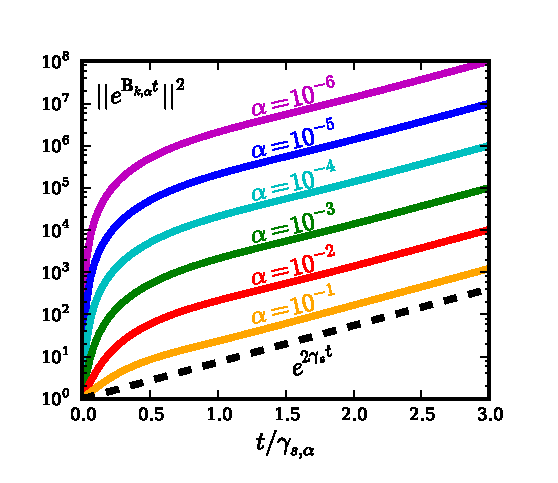
\includegraphics[width=0.45\textwidth]{max_en_growth}}
\caption{$G_{k,\alpha,\rm{max}}(t) = ||e^{\mathbf{B}_{k,\alpha} t}||^2$ for $k_x=0, k_y=1, \kappa=1$ for different values of the 2D adiabaticity parameter 
$\alpha$ compared to the energy growth $e^{2 \gamma_{s,\alpha,k} t}$ of the least stable eigenmode of  $\mathbf{B}_{k,\alpha}$. 
The time axis is normalized to $\gamma_{s,\alpha}$, which is different for each of the curves. This normalization makes the $e^{2 \gamma_{s,\alpha,k} t}$ line the same for all $\alpha$. 
$||e^{\mathbf{B}_{k,\alpha} t}||^2$ displays large non-exponential growth at early times that increases with decreasing $\alpha$.}
\label{max_en_growth}
\end{figure}

One explanation for this behavior is that non-normal matrices or operators have non-orthogonal linear eigenvectors. For the HW model, each Fourier matrix $\mathbf{B}_k$ has two eigenvectors associated
with it. They are complex and take the form:

\beq
\label{lin_eigen_form}
\psi_{k,q} = \left( \begin{array}{cc} n_k \\ k_\perp \phi_k \end{array} \right)_q {\rm sin} \left( k_x x \right) e^{i k_y y + i k_z z} 
\eeq
where the subscript $q$ takes the values of $1$ and $2$, representing the two eigenvectors for each $k$. The two eigenvectors are different in that they have a different complex ratio $n_k/\phi_k$.
The two eigenvalues have different growth rates (the real part), but the same frequency, though with opposite sign.
As $\alpha \to 0$, the two eigenvectors become less orthogonal -- more parallel or anti-parallel to one another. When the eigenvectors are nearly anti-parallel and initialized with finite amplitude,
their superposition, which constitutes the total system at $k$, may linearly evolve so that the norm of the superposition grows faster than either individual eigenvector. A paradigmatic illustration
of this may be seen in a review by Schmid~\cite{schmid2007}.

\section{The Effect of Non-Normality on Turbulence}

Linear non-normality is important for the effect it has on turbulence. It is most often cited as the sufficient condition for turbulence in subcritical systems, 
but it can also impact systems that have unstable linear eigenmodes like the HW system. Since certain superpositions of the linear eigenmodes can inject energy faster than the most unstable linear
eigenmode, there is the possibility that the energy injection into the turbulence is faster and at different wavenumbers than is suggested by linear eigenmode analysis. 
To understand this concept and show that it occurs in the nonlinear HW model, we compare the fastest growing linear eigenmode growth rate $\gamma_{s,k}$ to the turbulent growth rate $\gamma_{t,k}$. 
To define the turbulent growth rate in general and specifically for the HW model, we employ a Fourier-decomposed energy dynamics analysis~\cite{camargo1995,friedman2012b,friedman2013}. 
To do this, we take Eqs.~\ref{n_eq} and~\ref{phi_eq} and substitute the following:

\beqar
\label{subs_fourier}
n = \sum_{k} n_k \ {\rm sin} \left( k_x x \right) e^{i k_y y + i k_z z} \\
\phi = \sum_{k} \phi_k \ {\rm sin} \left( k_x x \right) e^{i k_y y + i k_z z},
\eeqar
where, again, $k$ stands for $(k_x,k_y,k_z)$.
Then, we multiply the resulting first equation by $n^*_{k'} \ {\rm sin} \left( k'_x x \right) e^{-i k'_y y - i k'_z z}$ and the second equation by 
$-\phi^*_{k'} \ {\rm sin} \left( k'_x x \right) e^{-i k'_y y - i k'_z z}$, take the volume integral and add the two equations together. The result is

\beqar
\label{Explicit_En_eqn}
\frac{1}{2} \diff{}{t} \left( |n_k|^2 + k^2_\perp |\phi_k|^2 \right) = -i k_y \kappa \phi_k n^*_k - \xi k_z^2 |n_k - \phi_k|^2 \nonumber \\
- D k^4_\perp \left( |n_k|^2 + k^2_\perp |\phi_k|^2 \right) + \sum_{k'} T(k,k'), \quad \quad
\eeqar
where, again, the energy $E_k$ is $\frac{1}{2} \left( |n_k|^2 + k^2_\perp |\phi_k|^2 \right)$, 
and the term $\sum_{k'} T(k,k')$ represents the nonlinear contribution (three-wave transfers between different $k$'s), 
which we do not write explicitly. This energy evolution equation may be written symbolically as

\beq
\label{dEdt_def}
\diff{E_k}{t} = \diff{E_{l,k}}{t} + \diff{E_{nl,k}}{t}
\eeq
where $\diff{E_{l,k}}{t}$ represents the terms that come from the linear terms in Eqs.~\ref{n_eq} and~\ref{phi_eq}, which are quadratic in the fluctuating
quantities $n_k$ and $\phi_k$ in Eq.~\ref{Explicit_En_eqn}. 
$\diff{E_{l,k}}{t}$ represents the injection of energy into the fluctuations from the free energy in the equilibrium gradients plus the dissipation from collisions and hyperdiffusion.
$\diff{E_{nl,k}}{t}$ represents $\sum_{k'} T(k,k')$ in  Eq.~\ref{Explicit_En_eqn} and comes from the nonlinear terms in 
Eqs.~\ref{n_eq} and~\ref{phi_eq}. The terms in $T(k,k')$ are triadic in the fluctuating quantities and
account for the energy exchange between fluctuations with different $k$'s. Furthermore, it is conservative: $\sum_{k} \diff{E_{nl,k}}{t} = \sum_{k,k'} T(k,k') = 0$.

Now, in quasi-steady state turbulence, the rate of net energy injection (or dissipation) into the fluctuations at each $k$ by the linear terms must be balanced by
the rate of energy removal (or deposition) from the nonlinear terms. This may be represented formally using growth rates:

\beqar
\label{steady_state}
\gamma_k \equiv  \displaystyle\lim_{T \to \infty} \frac{1}{T} \int_0^T \frac{dE_k/dt}{2 E_k} dt \nonumber \\
= \displaystyle\lim_{T \to \infty} \frac{{\rm{Log}}\left[ E_k(T)/E_k(0) \right]}{2 T} = 0
\eeqar
where the equality to zero clearly holds as long as the turbulence is in a steady or quasi-steady state.
From, Eqs.~\ref{dEdt_def} and~\ref{steady_state}, it follows that $ \gamma_k = \gamma_{l,k} + \gamma_{nl,k} = 0$.

We now associate the turbulent growth rate $\gamma_{t,k}$ discussed above with the linear rate of energy injection into the fluctuations $\gamma_{l,k}$ because $\gamma_{l.k}$
determines how fast and where in wavenumber space energy is injected into the turbulence.
$\gamma_{l,k}$, in other words, is the turbulence equivalent to the linear eigenmode growth rate $\gamma_{s,k}$~\cite{friedman2012b,terry2006b}. 
That is, in a linear simulation run for a sufficiently long time where transients die away, the calculation of $\gamma_{l,k}$ gives exactly $\gamma_{s,k}$.
Moreover, $\gamma_{l,k}$ is calculated from the spatial structures of the plasma state variables, so it is always well-defined, even in a turbulent plasma. 

A turbulent system, which can be decomposed into a linear eigenvector basis, has $\gamma_{t,k} \le \gamma_{s,k}$ if the system is normal. Recall that in normal systems, the maximal
energy growth is given by the most unstable linear eigenmode. In other words, maximal growth is achieved when the \emph{most stable} eigenmode has zero amplitude.
On the other hand, non-normal systems may grow faster when the more stable eigenmode has finite amplitude than when it has none (see Fig.~\ref{max_en_growth}). 
It is therefore possible for $\gamma_{t,k} > \gamma_{s,k}$ in non-normal systems. 

\begin{figure}
\centerline{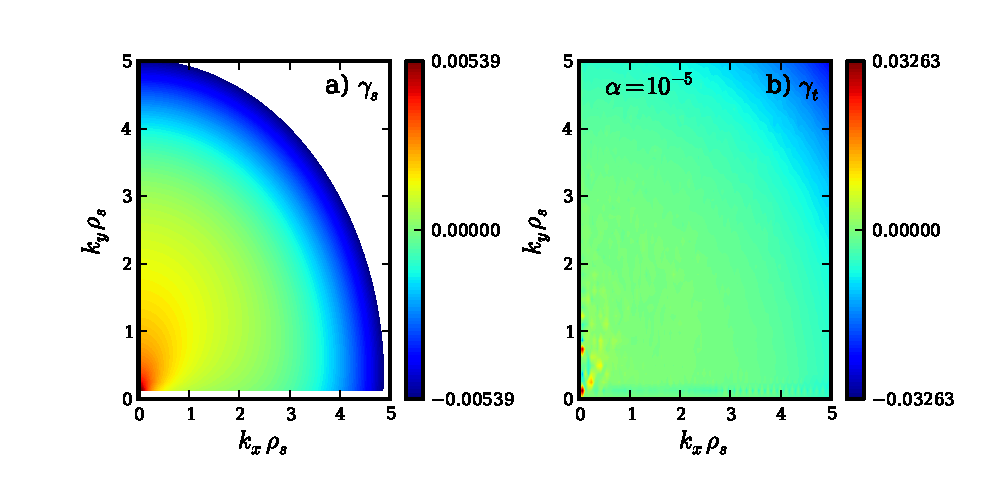
\includegraphics[width=0.52\textwidth]{alpha1e-5_gamma_s_t}}
\caption{a) The eigenmode growth rate spectrum $\gamma_{s,k}$ and b) the turbulent growth rate spectrum $\gamma_{t,k}$ for $\alpha = 10^{-5}, \kappa=1$. Note the different scales.}
\label{alpha1e-5_gamma_s_t}
\end{figure}

\begin{figure}
\centerline{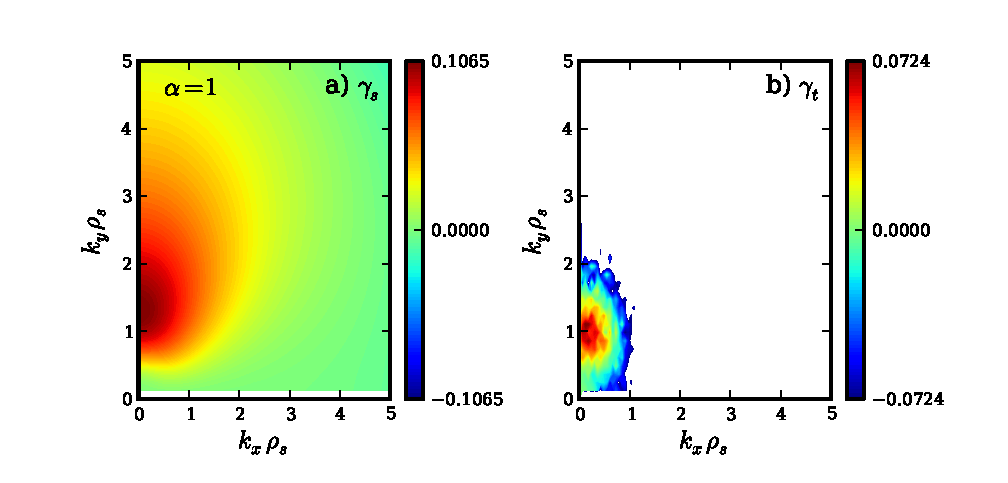
\includegraphics[width=0.52\textwidth]{alpha1_gamma_s_t}}
\caption{a) The eigenmode growth rate spectrum $\gamma_{s,k}$ and b) the turbulent growth rate spectrum $\gamma_{t,k}$ for $\alpha = 1, \kappa=1$.}
\label{alpha1_gamma_s_t}
\end{figure}

For the 2D HW model, we show
$\gamma_{s,k}$ and $\gamma_{t,k}$ for two different values of $\alpha$. In Fig.~\ref{alpha1e-5_gamma_s_t}, we show these growth rate spectra for $\alpha = 10^{-5}$, for which the system is
highly non-normal, and in Fig.~\ref{alpha1_gamma_s_t} for $\alpha = 1$, for which the system is very close to being normal. All calculations in this section use $\kappa=1$. 
Note the different scales used in all of the figures. In the highly
non-normal case, the turbulent growth rate is somewhat higher than the eigenmode growth rate for most values of $k_x,k_y$, and about 6 times higher where the spectrum peaks. For the more normal
case, in contrast, $\gamma_{t,k}$ is generally lower than $\gamma_{s,k}$, with the peak at nearly a factor of 2 less, with the peaks being at slightly different values of $k_y$.

\begin{figure}
\centerline{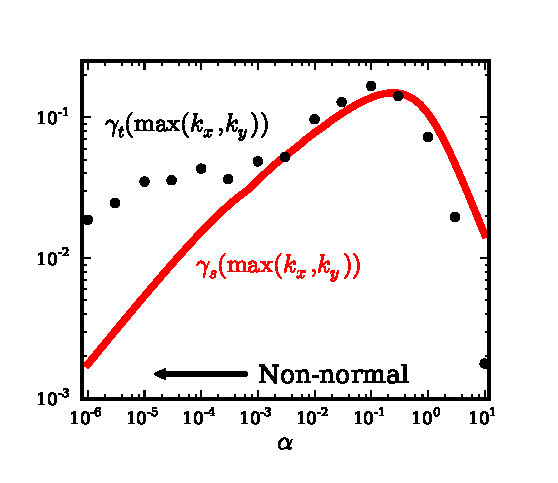
\includegraphics[width=0.4\textwidth]{gamma_max_vs_alpha}}
\caption{The eigenmode $\gamma_{s}$ and turbulent $\gamma_{t}$ growth rates as a function of $\alpha$, which controls the normality of the linear operator. All growth rates are peaks in $k_x-k_y$ space.}
\label{gamma_max_vs_alpha}
\end{figure}

We show the peak values for $\gamma_{s,k}$ and $\gamma_{t,k}$ in Fig.~\ref{gamma_max_vs_alpha} as a function of $\alpha$. The peak values always occur in $k$-space
at the lowest $k_x$ available to our system, corresponding to half of a period of a sine wave. The value of $k_y$ that gives the highest growth rate migrates upward as $\alpha$ increases,
as is clear from Figs.~\ref{alpha1e-5_gamma_s_t} and~\ref{alpha1_gamma_s_t}. Furthermore, as expected, when $\alpha$ is small ($\lesssim 10^{-3}$), $\gamma_{t,k} > \gamma_{s,k}$, with
$\gamma_{t,k} \gg \gamma_{s,k}$ as $\alpha \to 0$. Additionally, when $\alpha$ becomes larger and the system becomes more normal ($\gtrsim 10^{-1}$), $\gamma_{t,k} < \gamma_{s,k}$.

For both the normal and highly non-normal limits of the 2D HW model, $\gamma_{s,k}$ does a poor job of predicting $\gamma_{t,k}$ because $\gamma_{s,k}$ neglects the stable branch of the
dispersion relation -- the damped eigenmode. The importance of the stable eigenmode branch (or branches) 
has started to gain acceptance in the plasma community, although it has generally been used in normal
or nearly normal systems to explain turbulent saturation~\cite{terry2006b} ($\gamma_{t,k} < \gamma_{s,k}$). The case of highly non-normal turbulence and the associated increased turbulent excitation
hasn't been understood as well. In fact, simulation and analysis of the 3D HW model (and extended models) is an area in which others have seen the effects of strong non-normal transient growth
but have not realized them as such.


\begin{figure}
\centerline{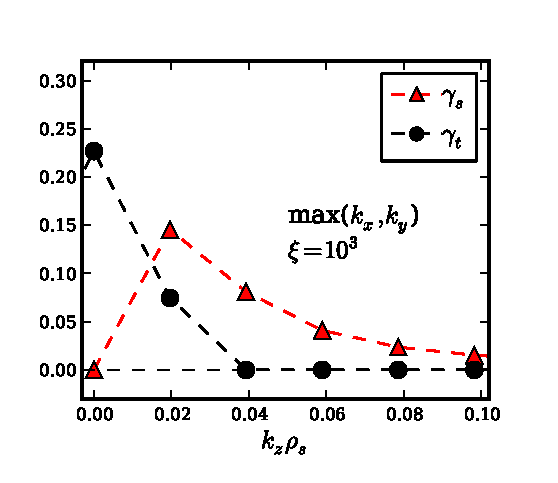
\includegraphics[width=0.4\textwidth]{gamma_max_vs_kz}}
\caption{The growth rates of the fastest growing eigenmode $\gamma_{s,k}$ and the of the turbulence $\gamma_{t,k}$ as a function of $k_z$ for the 3D HW model. The most remarkable feature is
that the turbulent growth rate peaks at $k_z=0$ despite the stability of all linear eigenmodes at $k_z=0$.}
\label{gamma_max_vs_kz}
\end{figure}

The 3D HW model nonlinear simulation has a fascinating property -- the turbulent energy injection is strongest at $k_z = 0$ despite the fact that there can be no unstable linear eigenmodes at $k_z=0$.
We show this in Fig.~\ref{gamma_max_vs_kz} using the eigenmode $\gamma_{s,k}$ and turbulent $\gamma_{t,k}$ growth rates, plotting them as a function of $k_z$.
The long-stated cause of this $k_z=0$ energy injection is a nonlinear instability, which was discovered by Biaskamp and Zeiler~\cite{biskamp1995} and explored further by Drake et al.~\cite{drake1995}. 
The nonlinear instability works as follows: magnetic-field-aligned ($k_z=0$) convective cells transport density across the equilibrium density gradient, setting up $k_z=0$ density structures. 
These structures are unstable to drift waves, which grow as a secondary instability.
The secondary drift waves, which have finite $k_z$, nonlinearly couple to one another and reinforce the original convective cells (or generate new ones), leading to self-sustainment.

Although the instability is a nonlinear instability, the first part of the mechanism -- the transport of background density by the convective cells -- is a linear one.
Biskamp and Drake understood this and wondered how there could be linear energy injection despite the fact that the linear eigenvectors are stable.
The answer to this came when Camargo et al.~\cite{camargo1998} stated that ``some properties of the drift-wave turbulence
previously attributed to nonlinear terms could also be strongly influenced by the nonnormal character of the linear system.'' Although Camargo et al. focused only on the 2D HW model,
based on this statement, it was likely apparent to them that the 3D HW nonlinear instability was a result of linear non-normality. 
Therefore, when $k_z=0$, no matter the value of $\xi$, the adiabaticity parameter $\alpha = k_z^2 \xi = 0$, meaning the linear matrix operator is highly non-normal and subject to transient growth.
So non-normal effects plays a role in the 3D HW system no matter what value of $\xi$ is chosen due to the presence of $k_z=0$ structures.

\section{Non-Modal Linear Technique To Calculate Turbulent Growth Rate}

In this section, we outline a procedure that uses quick and simple methods to approximate the turbulent growth rates $\gamma_{t,k}$.
We contend that the key to doing this is to successfully model the effect that the nonlinearities have on the linear (modal and transient) processes.
First, we note that the advective nonlinearity terms in Eqs.~\ref{n_eq} and~\ref{phi_eq} have the form of the state variable divided by a time $\tau_{nl} \sim (v_E k_\perp)^{-1}$. 
This nonlinear time scale is generally associated with the eddy turnover or decorrelation time. We therefore present a heuristic model of the nonlinearities 
as a randomizing force that acts on this characteristic nonlinear time scale. More specifically, this model is one in which 1) the turbulence begins as a random state, 
2) evolves linearly for a time $\tau_{nl}$, and 3) randomizes by nonlinear energy transfer, at which point the steps repeat.

This model can be used by starting with an ensemble of random initial conditions, evolving them linearly for a time $\tau_{nl}$, and
then taking the time and ensemble averaged growth rate of these curves.
In practice, this procedure can be greatly sped up and simplified. To see this, recall that the time evolution of the energy from an initial condition is

\beq
\label{E_t_from_u0}
E_k(t) = ||e^{\mathbf{B}_k t} u(0)||^2 = e^{\mathbf{B}_k t} u(0) u^{\dagger}(0) e^{\mathbf{B}_k^{\dagger}t}.
\eeq
Since we want to take the $\mathbf{u}(0)$ in the ensemble as random normalized vectors with uncorrelated components, it follows that~\cite{camargo1998}

\beq
\label{E_t_ensemble_avg}
\left< E_k(t) \right>_{{\rm{ens}}} = \frac{1}{2} {\rm{tr}} \{ e^{\mathbf{B}_k t} e^{\mathbf{B}^{\dagger}t} \},
\eeq
where the normalization is $||\mathbf{u}(0)||^2 = 1$. Mathematically, we define the non-modal growth rate $\gamma_{{\rm{nm}},k}$ as the time averaged instantaneous growth rate:

\beq
\label{gamma_nm_calc}
\gamma_{{\rm{nm}},k} = \frac{1}{\tau_{nl,k}} \int_0^{\tau_{nl,k}} \frac{\pdiff{E_k(t)}{t}}{2 E_k(t)} dt = \frac{1}{2 \tau_{nl,k}} \ {\rm{Log}} \left[ \frac{E_k(\tau_{nl,k})}{E_k(0)}\right].
\eeq
Next, we substitute the ensemble averaged energy calculated from Eq.~\ref{E_t_ensemble_avg} for $E_k(t)$, and set $E_k(0) = 1$ by our normalization. Then,

\beq
\label{gamma_nm}
\gamma_{{\rm{nm}},k} = \frac{1}{2 \tau_{nl,k}} \ {\rm{Log}} \left<  E_k(\tau_{nl,k}) \right>_{\rm{ens}}
\eeq
Now, in order to obtain a simple and quick prediction of $\gamma_{{\rm{nm}},k}$, we must estimate $\tau_{nl,k}$ without having to calculate it directly from a simulation. 
We thus invoke the conjecture of \emph{critical balance}, which posits that the nonlinear time scale equals the linear time scale at all spatial scales~\cite{schekochihin2012}. This is a fair
assumption in light of our discussion above, in which we derived the relation: $\gamma_{l,k} = - \gamma_{nl,k}$.

There are two fairly obvious linear time scales in the HW problem. First is the inverse of the linear eigenmode frequency $\omega_{s,k}$
-- the imaginary part of the eigenvalues of the linear matrix operator $\mathbf{B}_k$.
Recall that the imaginary part of the linear eigenvalues is the same for both eigenvalues of $\mathbf{B}_k$, so there is no question of which to use. We thus define the first non-modal
growth rate $\gamma_{\omega,k}$ as

\beq
\label{gamma_omega_def}
\gamma_{\omega,k} = \frac{\omega_{s,k}}{2} \ {\rm{Log}} \left< E_k(1/\omega_{s,k}) \right>_{\rm{ens}}.
\eeq
This growth rate is calculated by first finding $\omega_{s,k}$ of $\mathbf{B}_k$, and then inserting this into Eq.~\ref{gamma_omega_def} using the definition of 
$\left< E_k(1/\omega_{s,k}) \right>_{\rm{ens}}$ from Eq.~\ref{E_t_ensemble_avg}.

The second linear time scale that we may use is the inverse of the linear growth rate. However, the eigenvalues of $\mathbf{B}_k$ have different growth rates (real parts). 
Furthermore, we have argued that the eigenmode growth rates have little bearing on turbulence, especially for highly non-normal turbulence, 
so it would be innappropriate to use either of the linear eigenmode growth rates as a proxy for the nonlinear time scale.
Rather, we use the result itself, $\gamma_{{\rm{nm}},k}$, as the inverse of $\tau_{nl,k}$. Substituting $1/|\gamma_{{\rm{nm}},k}|$ for $\tau_{nl,k}$ in Eq.~\ref{gamma_nm_calc}, we get
a transcendental equation:

\beq
\label{trans_gamma_nm}
\gamma_{{\rm{nm}},k} = \frac{|\gamma_{{\rm{nm}},k}|}{2} \ {\rm{Log}} \left< E_k(1/|\gamma_{{\rm{nm}},k}|) \right>_{\rm{ens}}.
\eeq
We label this second non-modal growth rate $\gamma_{\gamma,k}$, and ultimately simplify this equation to

\begin{figure}
\centerline{\includegraphics[width=0.52\textwidth]{alpha1e-5_gamma_spec_compare}}
\caption{a) The eigenmode growth rate spectrum $\gamma_{s,k}$,  b) the turbulent growth rate spectrum $\gamma_{t,k}$, c) the non-modal growth rate spectrum $\gamma_{\omega,k}$ d) and the 
non-modal growth rate spectrum $\gamma_{\gamma,k}$ for the 2D HW model with $\alpha = 10^{-5}, \kappa=1$. Note the different scales.}
\label{alpha1e-5_gamma_spec_compare}
\end{figure}

\begin{figure}
\centerline{\includegraphics[width=0.52\textwidth]{alpha1_gamma_spec_compare}}
\caption{a) The eigenmode growth rate spectrum $\gamma_{s,k}$,  b) the turbulent growth rate spectrum $\gamma_{t,k}$, c) the non-modal growth rate spectrum $\gamma_{\omega,k}$ d) and the 
non-modal growth rate spectrum $\gamma_{\gamma,k}$ for the 2D HW model with $\alpha = 1, \kappa=1$.}
\label{alpha1_gamma_spec_compare}
\end{figure}


\beq
\label{gamma_pm2}
\left< E_k(1/|\gamma_{\gamma,k}|) \right>_{\rm{ens}} = e^{\pm 2},
\eeq
where if $\left< E_k(t) \right>_{\rm{ens}}$ first reaches $e^2$, $\gamma_{\gamma,k}$ is positive, and if it first reaches $e^{-2}$, $\gamma_{\gamma,k}$ is negative.
Therefore, finding $\gamma_{\gamma,k}$ amounts to a root-finding problem, which is not trivial, but is much simpler than a nonlinear simulation. 

We test both of these non-modal growth rates to see if either or both produce good approximations of $\gamma_{t,k}$, especially in comparison to $\gamma_{s,k}$. 
In Fig.~\ref{alpha1e-5_gamma_spec_compare}, we show the $\gamma_{\omega,k}$ and $\gamma_{\gamma,k}$ spectra for the 2D HW
model for $\alpha=10^{-5}$ along with the eigenmode and turbulent spectra ($\gamma_{s,k}$ and $\gamma_{t,k}$), which we already provided in Fig.~\ref{alpha1e-5_gamma_s_t}. We do the same for
$\alpha=1$ in Fig.~\ref{alpha1_gamma_s_t}. For the highly non-normal case ($\alpha = 10^{-5}$), $\gamma_{\omega,k}$ reproduces $\gamma_{t,k}$ in both magnitude and spectral shape. $\gamma_{\gamma,k}$
is not close in any respect to $\gamma_{t,k}$. On the other hand, for the nearly normal case ($\alpha=1$), $\gamma_{\omega,k}$ does not resemble $\gamma_{t,k}$. $\gamma_{\gamma,k}$ actually is
fairly similar to $\gamma_{s,k}$, but with a slightly decreased amplitude, making it a closer match to $\gamma_{t,k}$, though it is still not similar for all $k$.

\begin{figure}
\centerline{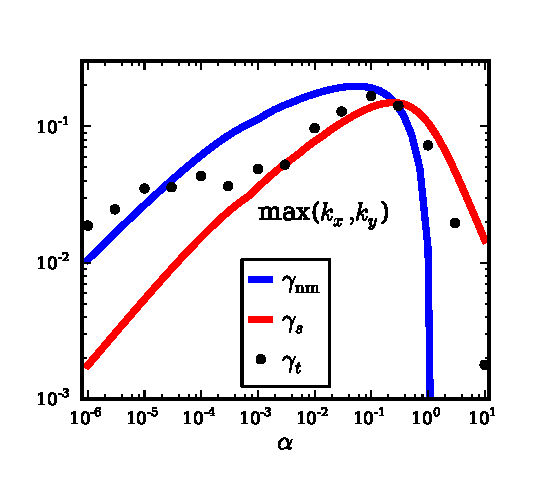
\includegraphics[width=0.45\textwidth]{gamma_max_with_nm}}
\caption{Comparison of the non-modal growth rates, $\gamma_{\omega,k}$ and $\gamma_{\gamma,k}$, to the eigenmode $\gamma_{s}$ and turbulent $\gamma_{t}$ growth rates as a function of $\alpha$
for the 2D HW model. All growth rates are peaks in $k_x-k_y$ space.}
\label{gamma_max_with_nm}
\end{figure}

We further test how well the maxima of the non-modal growth rates predict the maxima of the turbulent growth rates. We show the result in Fig.~\ref{gamma_max_with_nm}. For $\alpha < 10^{-3}$,
in which the system is fairly non-normal, $\gamma_{\omega,k}$ predicts $\gamma_{t,k}$ quite accurately. As the system becomes more normal, $\gamma_{t,k}$ and $\gamma_{\omega,k}$ diverge, with
$\gamma_{t,k}$ taking on values between $\gamma_{s,k}$ and $\gamma_{\omega,k}$, but generally closer to $\gamma_{s,k}$ for $\alpha \gg 10^{-3}$. 
This indicates that some assumption in our procedure doesn't work well for systems that are normal or nearly normal. Namely, our assumption
of complete randomization by the nonlinearities breaks down. Apparently, the nonlinearities only partially randomize the turbulence. For the most part, the turbulence at a given $k$ consists
primarily of the unstable eigenmode, while the stable eigenmode accounts for only a small amount of energy in the turbulence. Finally, $\gamma_{\gamma,k}$ is not useful in predicting $\gamma_{t,k}$.
It is closest to $\gamma_{t,k}$ for $\alpha \ge 1$, however, it only provides a slight improvement over $\gamma_{s,k}$ in this range.

\begin{figure}
\centerline{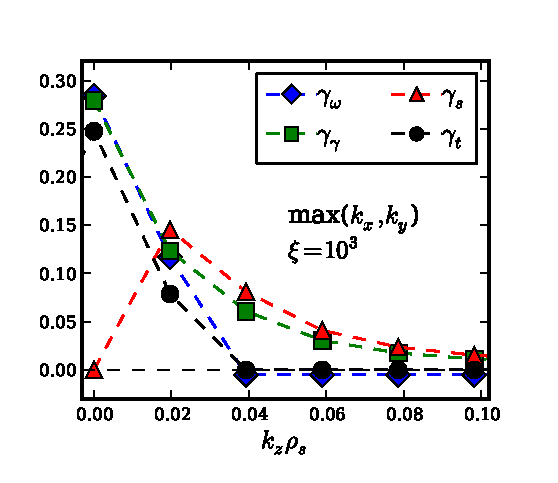
\includegraphics[width=0.4\textwidth]{gamma_max_vs_kz_with_nm}}
\caption{Comparison of the non-modal growth rates, $\gamma_{\omega,k}$ and $\gamma_{\gamma,k}$, to the growth rates of the fastest growing eigenmode $\gamma_{s,k}$ 
and the of the turbulence $\gamma_{t,k}$ as a function of $k_z$ for the 3D HW model. The non-modal growth rates correctly predict the growth rate dominance of the $k_z=0$ mode
despite the $k_z=0$ eigenmode stability.}
\label{gamma_max_vs_kz_with_nm}
\end{figure}

We do the same comparison for the 3D HW model as we did for the 2D HW model. However, there is one additional subtelty when considering the 3D model. In the 3D model, for $k_z=0$, the linear
eigenmode frequency is zero ($\omega_{s,k_z=0} = 0$), so $\gamma_{\omega,k_z=0}$ is not well defined (see Eq.~\ref{gamma_omega_def}). 
We could, in fact, make the argument that since $\omega_{s,k_z=0} = 0$, or by critical balance $\tau_{nl,k_z=0} \to \infty$, it would be proper to equate $\gamma_{\omega,k_z=0}$ with $\gamma_{s,k_z=0}$
since all transients die away in the long time limit. Rather, we use $\omega_{s,k_z=0.02}$ -- where $k_z=0.02$ is the lowest finite value of $k_z$ available to our system -- in place of
$\omega_{s,k_z=0}$ in the calculation of $\gamma_{\omega,k_z=0}$. We contend that the nonlinear instability, which most strongly couples $k_z=0$ and $k_z=0.02$ modes, has its time scale set
by the drift waves, not the convective cells, making $1/\omega_{s,k_z=0.02}$ a good proxy for $\tau_{nl,k_z=0}$. One may recall that the drift waves are actually secondary, and therefore, they feed
off of the $k_z=0$ density structures, so the appropriate scale length to use for $\omega_{s,k_z=0.02}$ is not given by $\kappa$, but by the scale length of the density structures. We don't deal
with this complication and assume the scale length of the fluctuating density structures is the same as the background.

Despite these complications at $k_z=0$, our non-modal method of calculating $\gamma_{\omega,k}$ approximates $\gamma_{t,k}$ remarkably well as seen in Fig.~\ref{gamma_max_vs_kz_with_nm}.
Most importantly, it correctly predicts that $\gamma_{\omega,k_z=0} > 0$ and $\gamma_{\omega,k_z=0} > \gamma_{\omega,k_z \ne 0}$. Therefore, non-modal calculations explain why the 3D HW model
is dominated by the nonlinear instability rather than a linear drift wave instability. Simply put, transient growth is strongest at $k_z=0$, so the nonlinear instability is energetically
favored over the linear instability. Again, $\gamma_{\gamma,k}$ does not provide enough accuracy to warrant its use.

\section{Prediction of Control Parameter for Subcritical Turbulent Onset}

In both hydrodynamic and plasma systems, it is important to be able to predict the smallest value of a control parameter for which the system will become turbulent. 
The control parameter is different for different systems (and models of those systems), and there may be several control parameters for a particular problem. When $d$ control parameters exist in a model, 
there is not a single point in the parameter space at which the system bifurcates to turbulence, rather, there is a $d-1$ manifold that separates the laminar and turbulent states.
In many hydrodynamic systems driven turbulent by shear flow, there is generally a single control parameter -- the Reynold's number $Re$~\cite{drazin1981}.
In plasmas, there are often multiple control parameters. For instance, kinetic solar wind turbulence models have two: $\beta$ and $T_\perp/T_\para$~\cite{camporeale2010}). One kinetic turbulence in the
core of a tokamak has three: $\gamma_E$ (the normalized perpendicular flow shear), $R/L_T$ (the inverse ion temperature gradient scale length normalized to the major radius), and $q/\epsilon$
(the ratio of the magnetic safety factor to the inverse aspect ratio)~\cite{highcock2012}.

For normal systems, turbulence will be excited when the control parameter becomes large enough such that one of the linear eigenmodes becomes unstable (the real part of the eigenvalue crosses into the
right half of the complex plane). In general, this is not the case for non-normal systems. In many non-normal systems, turbulence can be sustained when all linear eigenmodes are stable --
the case of subcritical turbulence. 

\begin{figure}
\centerline{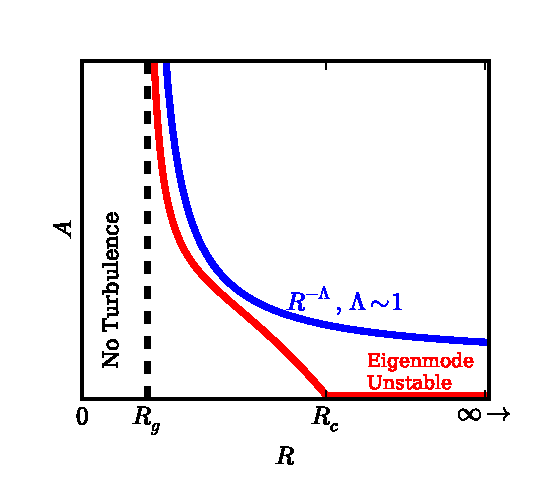
\includegraphics[width=0.4\textwidth]{subcritical_diagram}}
\caption{Diagram of a control parameter $R$ versus perturbation amplitude $A$ for two subcritical systems. The first curve (top blue one with $R^{-\Lambda}$ label) represents a system with no
eigenmode instability for any $R$, but which is stable to finite amplitude perturbations for $R > R_g$. 
The second (bottom red one with label of ``Eigenmode Unstable'') represents a system with a linear eigenmode instability for $R \ge R_c$, and finite amplitude
instability for $R_g < R < R_c$.}
\label{subcritical_diagram}
\end{figure}

Subcritical systems fall into two categories: those that have stable eigenmodes for all values of the control parameter, and those that have unstable eigenmodes
when the control parameter becomes large enough. We illustrate these two categories with a diagram in Fig.~\ref{subcritical_diagram}. 
The upper curve represents the first kind of subcritical system in which no unstable eigenmodes exist for any value of $R$. In this
case, there is some transitional value of $R$, labeled $R_g$, below which turbulence cannot occur. When a perturbation with amplitude above the line occurs in the system due to external input or noise, 
turbulence will be excited. Perturbations with amplitude below the line will decay away. Clearly, the higher the value of $R$, the smaller the perturbation needs to be to excite turbulence.
Experimental evidence and theoretical arguments show this curve should have a $R^{-\Lambda}$ dependence, with $\Lambda \sim 1$~\cite{grossmann2000}.
A paradigmatic example of this kind of system is Hagen-Poisuille pipe flow -- flow in a cylindrical pipe with a parabolic flow profile -- for which $R_g \approx 2000$.

The lower curve represents the second kind of subcritical system. Above a critical value of the control parameter $R_c$, the system is linearly unstable. But, for $R_g < R < R_c$, the system is
unstable to finite amplitude perturbations, or ``nonlinearly'' unstable. A paradigmatic example of this is Poissuille channel flow -- the rectangular analog of pipe flow -- for which
$R_c = 5772$ and $R_g \approx 1000$~\cite{grossmann2000}. Most subcritical magnetically-confined plasma systems fall into this category. It is perhaps easy to be fooled into believing that the turbulence
in such systems is due to eigenmode instability. In either case, one of the most important predictions is the minimum turbulent control parameter $R_g$.

The HW model in an unsheared magnetic slab is not subcritical in either the 2D or 3D cases, as implied by Figs.~\ref{gamma_max_vs_alpha} and~\ref{gamma_max_vs_kz}. It is subcritical in a highly sheared
magnetic field~\cite{drake1995}, but the eigenmodes of the linear operator in that case are not sinusoidal, making our non-modal analysis more difficult. Biskamp et al., however, artificially modified the
3D HW model to remove the linear drive by taking the $z$ average of the $\kappa \pdiff{\phi}{y}$ term in Eq.~\ref{n_eq}, effectively eliminating the $k_z \ne 0$ drive. This leaves only the $k_z = 0$
component of the drive term. Since the $k_z = 0$ eigenmodes are stable but $k_z = 0$ structures can access the free energy (positive $\gamma_t$ in Fig.~\ref{gamma_max_vs_kz}), this system is subject
to subcritical turbulence.

We show that the system is subcritical in Fig.~\ref{init_en_ev} by plotting the energy versus time for fluctuations that are initialized with different amplitudes. When the fluctuations are initialized
with high enough amplitude, the system eventually becomes turbulent. Otherwise, the fluctuations grow transiently, but do not reach high enough amplitude for the nonlinearities to bootstrap the process,
so they decay away. The finite amplitude turbulence threashold, as described above, is the key indicator of subcritical turbulence.

\begin{figure}
\centerline{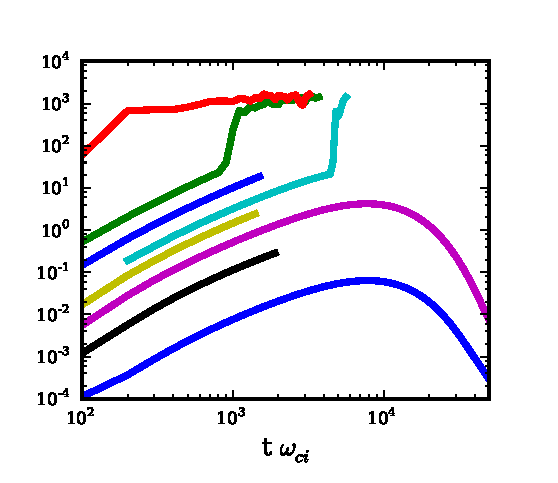
\includegraphics[width=0.4\textwidth]{init_en_ev}}
\caption{Total energy evolution of fluctuations of the modified 3D HW model where the initial perturbations are set to different amplitudes. All initial perturbations are initialized randomly in
the $y$ and $z$ directions and with a Guassian in the $x$ direction. There is a critical initial amplitude threashold above which turbulence develops and maintains itself
and below which turbuelence never develops and the fluctuations decay away. This indicates that the modified model is subject to subcritical turbulence.}
\label{init_en_ev}
\end{figure}


\begin{acknowledgments}
This work was supported by the National Science Foundation (Grant PHY-1202007)
\end{acknowledgments}

%%%%%%%%%%%%%%%%%%%%%%%%%%%%%%%%%%%%%%%%%%%%%%%%%%%%%%%%%%%%%%%%%%%%%%%%%%%

%\bibliographystyle{phaip}
\bibliography{refs}

\end{document}
